\section{Verifizierung des Reglers an der Regelstrecke}
Die letztendliche Aufgabe besteht darin einen Regler zu entwerfen, damit der Würfel auf einer Kante balanciert. Hierfür wird ein linear quadratisch optimaler Regler entworfen, wobei die Gewichtsmatrizen
\begin{equation}
\bs{Q} = \begin{bmatrix}
\varphi^{-2}_{max} & 0 & 0 \\
0 & u^{-2}_{K,max} & 0 \\
0 & 0 & u^{-2}_{R,max}
\end{bmatrix}
\hspace{35pt}
\bs{R} = \begin{bmatrix} T^{-2}_{M,max} \end{bmatrix}
\end{equation}
verwendet werden. Daraus resultiert das Gütekriterium
\begin{equation}
J = \sum^{\infty}_{k=0}\left( \frac{\varphi^2}{\varphi^2_{max}} + \frac{u_K^2}{u^2_{K,max}} + \frac{u^2_{R}}{u^2_{R,max}} + \frac{T_M^2}{T^2_{M,max}}\right)\,.
\end{equation}
Somit werden der Zustandsvektor und die Stellgröße quadratisch über ihren maximalen Wert minimiert. Der daraus resultierende Regelkreis besitzt die Eigenwerte
\begin{equation}
\lambda_1 = 0,7895 \hspace{35pt} \lambda_{2,3} = 0,8830 \pm 0,0087j
\end{equation}
und ist somit asymptotisch stabil. Im nächsten Schritt wird der Regler an der realen Regelstrecke validiert. Die folgende Abbildung zeigt den Verlauf der Zustands- und Stellgröße, wobei das System bei dem Zeitpunk $t\approx 15$ durch eine äußere Störung erregt wurde.
\begin{figure}[h!]
\centering
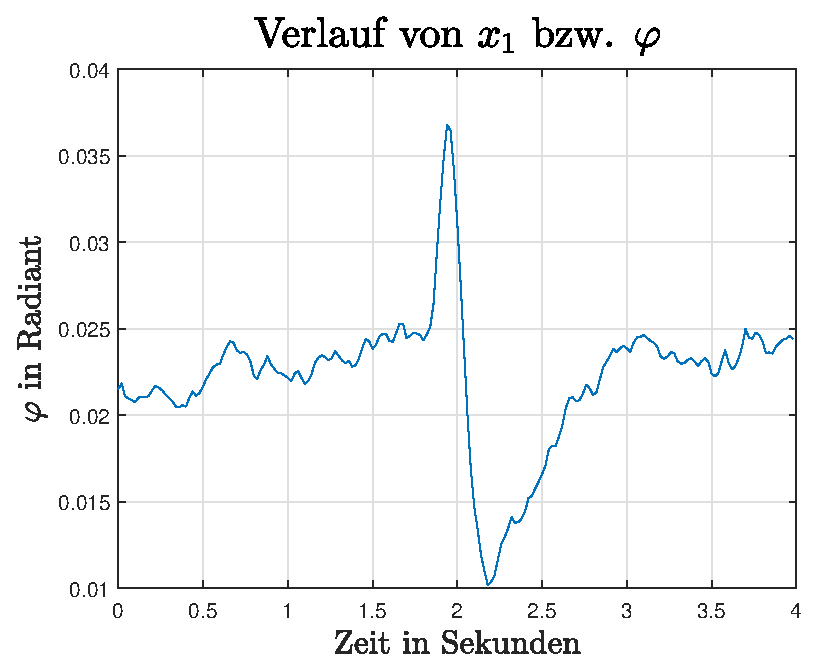
\includegraphics[width=0.45\linewidth]{img/edge_exp1_phi.eps}
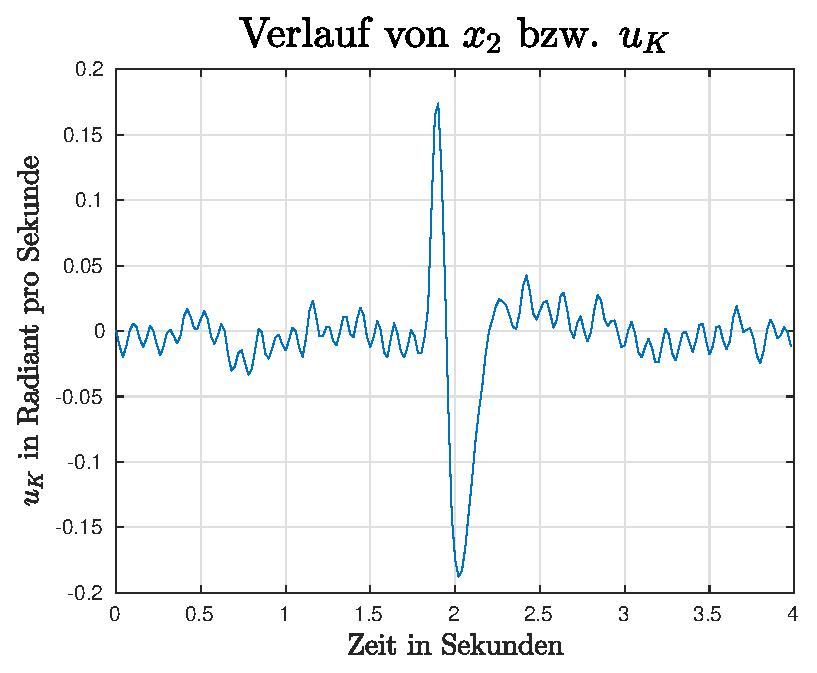
\includegraphics[width=0.45\linewidth]{img/edge_exp1_uk.eps}
\vspace{0.5cm}

\includegraphics[width=0.45\linewidth]{img/edge_exp1_ur.eps}
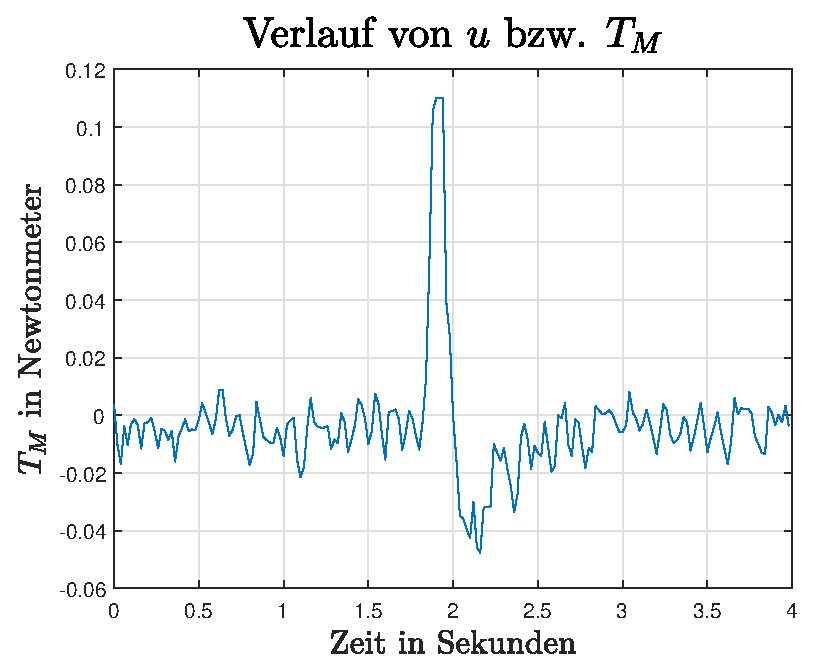
\includegraphics[width=0.45\linewidth]{img/edge_exp1_tm.eps}
\end{figure}

Die Abbildungen zeigen, dass der Regler das System nicht in die Ruhelage $\bs{x}=\bs{0}$ überführt, sondern die Schwungmasse mit konstanter Geschwindigkeit rotiert. Dieser Umstand ist darauf zurückzuführen, dass der Zustandsvektor mit einem systematischen Messfehler erfasst wird. Im Modell wird diese Gegebenheit durch die Einführung der Zustandsgrößen
\begin{equation}
\bs{\hat{x}} = \begin{pmatrix}
\hat{\varphi} \\ \hat{u}_K \\ \hat{u}_R
\end{pmatrix}
\end{equation}
erfasst, welche die jeweiligen Messabweichungen darstellen. Der Ausgangsvektor $\bs{y}$ stellt die Messwerte dar und wird durch die Summe des ursprünglichen Zustandvektors $\bs{x}$ und der Messabweichungen $\bs{\hat{x}}$ berechnet. Aus diesen Überlegungen ergibt sich für den offenen Regelkreis das System
\begin{equation}
\textfrak{D}_0 \equiv \left\{ \begin{split}
\bs{x}_o(k+1) &= \underbrace{\begin{bmatrix}
\bs{A} & \bs{0}^{3x3} \\ \bs{0}^{3x3} & \bs{I}^{3x3}\end{bmatrix}}_{\equiv \bs{A}_o}\cdot \underbrace{\begin{bmatrix}
\bs{x} \\ \bs{\hat{x}}
\end{bmatrix}}_{\equiv \bs{x}_0}(k) + \underbrace{\begin{bmatrix}
\bs{b} \\ \bs{0}^3 \end{bmatrix}}_{\equiv \bs{b}_o} \cdot u(k)
\\
\bs{y}(k) &= \underbrace{\begin{bmatrix}
\bs{I}^{3x3} & \bs{I}^{3x3}\end{bmatrix}}_{\equiv \bs{C}_o}\cdot \bs{x}_o(k)
\end{split}
\right. \,.
\end{equation}
Das Reglergesetz ergibt sich nun aus dem Produkt des Reglervektors $\bs{k}^T$ und des Ausgangsvektors $\bs{y}$.
\begin{equation}
u = \bs{k}^T\cdot \bs{y} = \bs{k}^T \cdot (\bs{x} + \bs{\hat{x}}) = \underbrace{\begin{bmatrix}
\bs{k}^T & \bs{k}^T
\end{bmatrix}}_{\equiv \bs{k}^T_o} \cdot \bs{x}_o
\end{equation}
Hiermit kann der Regelkreis geschlossen werden und es resultiert das System
\begin{equation}
\overline{\textfrak{D}}_o = \left\{ \begin{split}
\bs{x}_o(k+1) &= \begin{bmatrix}
\bs{A}-\bs{b}_o\bs{k}^T_o & -\bs{b}_o\bs{k}^T_o \\
\bs{0}^{3x3} & \bs{I}^{3x3}
\end{bmatrix}\cdot \bs{x}_o(k)
\\
\bs{y}(k) &= \bs{C}_o\cdot \bs{x}_o(k)
\end{split}\right.
\,.
\end{equation}
Für den geschlossenen Regelkreis ergeben sich die Eigenwerte
\begin{equation}
\lambda_1 = 0,7895 \hspace{35pt} \lambda_{2,3} = 0,8830 \pm 0,0087j \hspace{35pt} \lambda_{4,5,6} = 1
\,.
\end{equation}
Diese zeigen, dass die urpsrünglichen Eigenwerte erhalten bleiben und somit die Eigenbewegung nach wie vor stabilisiert wird. Die zusätzlichen Eigenwerte $\lambda_{4,5,6}=1$ sind den Messabweichungen zuzuordnen, welche als konstant modelliert wurden. Hieraus lässt sich folgern, dass der geschlossene Regelkreis als lineares System für beliebige Messabweichungen stabil ist, insofern diese nicht von einem instabilen Vorgang verursacht werden. Um den Einfluss der Messabweichungen auf die Trajektorie $\bs{x}$ zu ermitteln wird das System $\overline{\textfrak{D}}_o$ in die kanonische Normalform transformiert.
\begin{equation}
\tilde{\overline{\bs{A}}}_o = \bs{V}^{-1}_o\overline{\bs{A}}_o\bs{V}_o = \begin{bmatrix}
\lambda_1 & & & \\
 & \lambda_2 & & \\
 & & \ddots & \\
 & & & \lambda_6
\end{bmatrix}
\hspace{35pt} 
\bs{x}_o = \bs{V}_o\cdot \tilde{\bs{x}}_o
\end{equation}
Interessant ist hierbei die Form der Transformationsmatrix
\begin{equation}
\bs{V}_o = \begin{bmatrix}
\bs{V} & \begin{matrix} 0 & 0 & 0 \\ 0 & 0 & 0 \\ \gamma_1 & \gamma_2 & \gamma_3 \end{matrix} 
\\ \bs{0}^{3x3} & \bs{I}^{3x3}
\end{bmatrix}
\,.
\end{equation}
Zunächst geht aus den unteren drei Zeilen hervor, dass es sich bei den Messabweichungen $\bs{\hat{x}}$ um kanonische Zustandsvariablen handelt. Des weiteren bleiben die Eigenvektoren $\bs{V}$ des ursprünglichen Systems $\overline{\textfrak{D}}$ und somit auch dessen Eigenbewegung erhalten. Die Messabweichungen wirken lediglich über die Faktoren $\gamma_i$ auf die Geschwindigkeit $u_R$ des Schwungmasse ein. Unter der Annahme, dass die Messabweichungen konstant sind, führen diese zu einer verbleibenden Bewegung der Schwungmasse. Deshalb muss die vorherige Stabilitäsaussage auf das Gebiet der Zustands- und Stellgrößen begrenzt werden für welche die Stellgröße nicht begrenzt ist. Beispielsweise kann das System nicht mehr stabilisiert werden, wenn der Messfehler so groß ist, dass $\bs{\gamma}\cdot \bs{\hat{x}}$ die maximale Drehzahl des Motors überschreitet.

Da der Winkel $\varphi$ nach wie vor asymptotisch stabil ist entspricht der Endwert der gemessenen Größe $\bs{y}(1)$ der Messabweichung.
\begin{equation}
\bs{y}(1) = \varphi + \hat{\varphi} \rightarrow \lim_{k\rightarrow\infty}\bs{y}(1) = \hat{\varphi}
\end{equation}
Deshalb wird zunächst die Messabweichung $\hat{\varphi}$ bestimmt und in einem anschließenden Versuch korrigiert. Nach dem Modell ist zu erwarten, dass die Schwungmasse nahe zum Stillstand kommt. Dies ist darin begründet, dass lediglich die Messabweichung $\varphi$ korrigiert wird, diese allerdings den größten Einfluss auf den Endwert des Systems hat.
\begin{figure}[h!]
\includegraphics[width=0.45\linewidth]{img/edge_exp2_phi.eps}
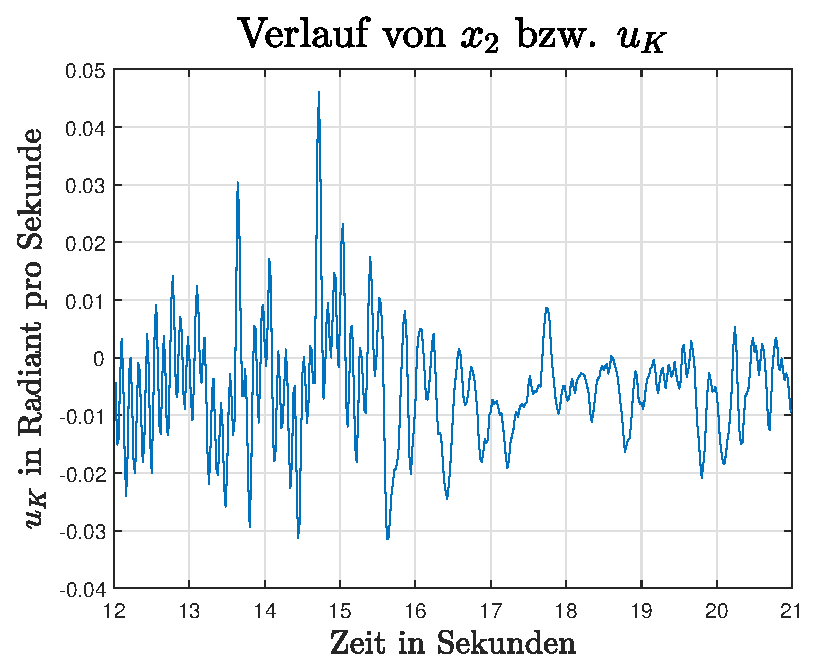
\includegraphics[width=0.45\linewidth]{img/edge_exp2_uk.eps}
\end{figure}
\begin{figure}[h!]
\includegraphics[width=0.45\linewidth]{img/edge_exp2_ur.eps}
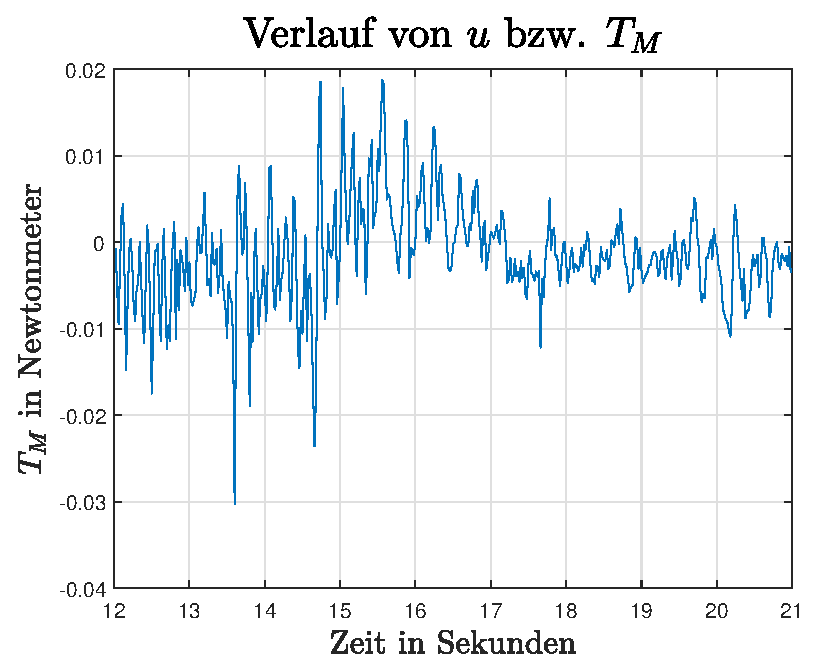
\includegraphics[width=0.45\linewidth]{img/edge_exp2_tm.eps}
\label{plot_edge_exp2}
\caption{Verlauf der Zustandsgrößen bei korrigierten Messabweichungen}
\end{figure}
\newpage
Abbildung (\ref{plot_edge_exp2}) zeigt den Verlauf der Zustandsgrößen, wobei zu dem Zeitpunkt $t=15$ die Messabweichung korrigiert wurde. Daraufhin nimmt die Geschwindigkeit $u_R$ der Schwungmasse deutlich ab.
